\chapter{An\'alisis del sistema}
\section{Identificaci\'on de problemas y oportunidades b\'asicas}
En el estudio del sistema, se encontraron los siguientes problemas:%
\\%
\begin{itemize}
	\item El sistema debe ser flexible y parametrizable.%
	\item El volumen del flujo de datos es muy grande.%
	
	
\end{itemize}%
%
\begin{figure}[htbp]
%centering es para centrar la imagen
	\centering
%aca es donde se incluye la imagen, se da el ancho(width), \textwidth significa que con repescto al tamano del
%texto y luego la ruta, relativa siempre es decir, a partir de donde se esta, como images esta ahi
%dentro, solo se usa desde images y ojala nada de espacios en el nombre de la imagen
		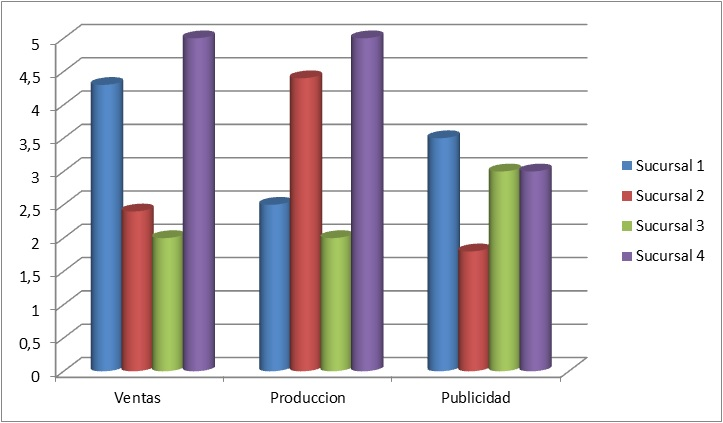
\includegraphics[width=0.60\textwidth]{images/Eficienciadelasucursal.jpg}
%el caption es para el texto que aparece debajo de la imagen
	\caption{Eficiencias de las sucursales}
%label es para darle una referencia, por ejemplo si uno dice "como se puede ver en la imagen a1"
	\label{fig:eficienciasucursales}
\end{figure}%
%
\section{Evaluaci\'on del beneficio del proyecto}
Lo beneficios de el sistema de informaci\'on que se va a implementar nos permitir\'a consultar, observar y verificar la informaci\'on de la compa\~n\'ia en tiempo real y efectiva, de tal forma que estos procesos puedan ser flexibles y f\'acil de manejar para el usuario, esto nos lleva a que se Incrementara  el entendimiento del uso de las Tecnolog\'ias de Informaci\'on en la organizaci\'on y posteriormente  incrementar las ventas; para llevar esto a cabo, es necesario ser el primero en proporcionar informaci\'on a clientes potenciales . y mantener una relaci\'on con ellos a trav\'es de informaci\'on permanente.%
%
\subsection{?`Vale la pena trabajar en este proyecto?}
Hoy en d\'ia se esta tomando conciencia de la importancia dentro de las organizaciones de manejar los ambientes de negocio implementando un sistema de informaci\'on, lo fundamental para una compa\~n\'ia es un mercado globalizado a nivel competitivo, que tanto la estrategia de negocios y estrategias tecnol\'ogicas est\'en bajo un mismo esquema.%
\\%
\\%
\subsection{?`Solucionar\'a los problemas?}
Uno de los principales inconvenientes de la organizaci\'on es que tiene gran cantidad de quejas y opiniones de los clientes esto lleva a que no se tenga en cuenta las opiniones de los clientes por ser una fuente de datos muy grande por eso se realizara este sistema, ya que el CRM es un sistema muy efenctivo en procesos frente al cliente por eso se implemetara, y esto sera para generar una mejor atecion al cliente, trato de todos los datos generando reportes y estadisticas.%
%
\subsection{Agregar valor al proceso}
Se agrega valor en los siguientes aspectos:%
\begin{enumerate}
	\item Proporcionando informacion adicional para la alta gerencia la cual ayuda para la toma de decisiones.
	\item Identificando inconvenientes que si resuelven y mejora la competencia y el incremento de las venta.
	\item Identificando las oportunidades de mejora en todas las \'areas.
\end{enumerate}%
%
\section{Dominio del problema}
El sistema que es implementado de forma sencilla no tan complejo ya que son pocos procesos que intervienen; siendo as\'i un sistema con 3 actores directos que son los comunity managers, los operadores del contact center y la organizaci\'on (due\~no de las campa\~nas del social media) a quien se le va a gestionar sus redes sosciales, en el que puede llegar a derivarse en altos niveles directivos y analistas de mercados. Actores indirectos son la otra faceta de este sistema y est\'a con formado por los clientes de la organizacion del social media, es decir, por dar un ejemplo: McDonalds necesita monitorear su impacto con sus clientes en las redes sociales; McDonalds se convierte en cliente del sistema y sus clientes van a hacer el objetivo de monitorizaci\'on.
%
%
\section{An\'alisis de los procesos del negocio}
Los principales procesos est\'an identificados de la siguiente manera:%
	\begin{itemize}
		\item Campa\~nas.
		\item Satisfacci\'on al cliente.
	\end{itemize}
\subsection{Campa\~nas:}
Se realizan campa\~nas para las diferentes tareas en la organizaci\'on, tales como comunicados, informaci\'on, aperturas, promoci\'on de productos y promoci\'on de empleos entre otras.%
%
\subsection{Satisfacci\'on al cliente:}Se realiza seguimiento en cuanto al servicio al cliente en aspectos como atenci\'on, calidad en productos, aseo, etc.%
%
\section{Marco Referencial}
%
\subsubsection{CRM} Costumer Relationship Manager es una estrategia de negocios dirigida a entender, anticipar y responder a las necesidades de los clientes actuales y potenciales de una empresa para poder hacer crecer el valor de la relaci\'on..%
\\%
\\%
CRM engloba 2 conceptos, el CRM hace tanto referencia a la estrategia de negocio focalizada hacia el cliente, como a toda las aplicaciones inform\'aticas, tanto software como hardware conocidas como front office , necesarias para procesar, analizar y exponer la informaci\'on resultante para medir y retroalimentar la estrategia de negocio desarrollada..%
\\%
\\%
Existen multitud de definiciones acerca del CRM que expresan la esencia de la anterior definici\'on, a continuaci\'on se exponen unas cuantas de ellas:%
\\%
\begin{itemize}
	\item Consiste en una estrategia de la organizaci\'on en la cual centra sus esfuerzos en el conocimiento de sus clientes, detectando sus necesidades, aumentando su grado de satisfacci\'on, incrementando su fidelidad a la empresa e incrementando la rentabilidad o beneficios del cliente a la empresa, mediante el an\'alisis de las informaciones extraidas por los clientes desde los diferentes canales o medios de comunicaci\'on.
	\item Se refiere a aquellas aplicaciones que las empresas pueden utilizar para administrar todos los aspectos de sus encuentros con los clientes. Un sistema CRM puede incluir todo, desde tecnolog\'ia para la recolecci\'on de datos en las llamadas telef\'onicas del \'area de ventas, hasta sitos web de autoservicio donde los clientes pueden aprender acerca de los productos y de su compra, o el an\'alisis de los clientes y los sistemas de administraci\'on de campa\~na.
	\item Es una estrategia general que permite a la empresa contactarse en forma eficiente con sus clientes. As\'i las soluciones CRM integran las tecnolog\'ia de la informaci\'on TI junto a la telefon\'ia para que las compa\~n\'ias puedan identificar, atraer y aumentar la retenci\'on de clientes fieles a trav\'es de la administraci\'on de dicha raz\'on.
	\item es un concepto gen\'erico en el que se denomina a las diversas soluciones de hardware y software que se est\'an ofreciendo hoy en el mercado y, se centra en lo que estas empresas llaman el "front office" que integra a las \'areas de ventas, marketing, publicidad, Internet, canales, etc. En conclusi\'on, es la nueva generaci\'on inform\'atica y, se enfoca en las soluciones de negocios, ya que hasta hace poco estas empresas de hardware y software ofrec\'ian en este campo solo productos aislados. La diferencia es que hoy se ha logrado integrar soluciones completas.
\end{itemize}
\subsubsection{Metolog\'ia de desarrollo \'agil } son m\'etodos de ingenier\'ia del software basados en el desarrollo iterativo e incremental, donde los requerimientos y soluciones evolucionan mediante la colaboraci\'on de grupos auto organizados y multidisciplinarios. Existen muchos m\'etodos de desarrollo \'agil; la mayor\'ia minimiza riesgos desarrollando software en lapsos cortos. El software desarrollado en una unidad de tiempo es llamado una iteraci\'on, la cual debe durar de una a cuatro semanas. Cada iteraci\'on del ciclo de vida incluye: planificaci\'on, an\'alisis de requerimientos, dise\~no, codificaci\'on, revisi\'on y documentaci\'on. Una iteraci\'on no debe agregar demasiada funcionalidad para justificar el lanzamiento del producto al mercado, pero la meta es tener una "demo" (sin errores) al final de cada iteraci\'on. Al final de cada iteraci\'on el equipo vuelve a evaluar las prioridades del proyecto.%
\subsubsection{Community Manager}
%
El responsable de la comunidad virtual, digital, en l\'inea o de internet, es quien act\'ua como auditor de la marca en los medios sociales; o gestor (también llamado en inglés como community manager) 1 cumple un nuevo rol dentro de la mercadotecnia, la Publicidad Online y la documentación, pues es una profesión emergente al igual que lo es el Record Manager.
Así, un Community Manager es la persona encargada o responsable de sostener, acrecentar y, en cierta forma, defender las relaciones de la empresa con sus clientes en el ámbito digital, gracias al conocimiento de las necesidades y los planteamientos estratégicos de la organización y los intereses de los clientes. La figura se remonta al origen de las comunidades virtuales como "The well" y luego siguió teniendo relevancia en el ámbito de las listas de distribución, los grupos de noticias y los foros web.
Crear, analizar, entender y direccionar la información producida para las redes sociales, monitorear acciones que se ejecutan, crear estrategias de comunicación digital, entre otras tantas, son las funciones de un Community Manager, con un único objetivo que será establecer una comunicación que lejos de silenciar, censurar o ignorar a sus clientes, sea transparente, abierta y honesta, acercando nuevos públicos afines con la marca; permitiendo apalancar las posibilidades de un nuevo modelo de “innovación Abierta”, ofreciendo así nuevas formas de comunicación más relevantes en las que en cliente se sienta parte activa de la organización”
\section{CRM como soluci\'on adecuada}
%
La necesidad del negocio se puede resumir en los siguientes puntos:%
%
\begin{itemize}
\item Busqueda de la satisfaccion de el cliente por medio de los comentarios echos por ellos.
\item Gesti\'on y soporte de quejas,reclamos,suerencias, cometarios etc, de cliente.
\item Control y seguimiento de las quejas,reclamos,suerencias, cometarios.
\item Estadisticas y reportes de quejas,reclamos,suerencias, cometarios.
\end{itemize}
%
Teniendo en cuenta esto, la soluci\'on m\'as acertada es la implementaci\'on de un CRM, debido a las caracter\'isticas mencionadas anteriormente.%
\\%
\\%
Un sistema CRM permite tener un analisis de las necesidades del cliente por ende se realiza este sistema ya que gestiona y soporta las quejas, reclamos, suerencias, cometarios realizados por los clientes y esto se manipularan con el proposito de mejorar la organizacion dependiendo de las quejas hechas por los clientes de la organizaci\'on y asi llegar a un total control de todas las necesidades de los clientes, y asi mostrado por medio de estadisticas, graficos y reportes.
\\%
Con la automatizacion  de estos procesos por medio del CRM Buscaremos:
%
\begin{itemize}
	\item Mejorar el flujo de procesos. 
	\item Obtener un mejor an\'alisis y respuestas.
	\item Facilitar el servicio al cliente.
	\item Satisfaser en totalidad las necesidades de los clientes.
\end{itemize}
%

